\begin{center}
  \textsf{Листок 2.}
\end{center}
\vspace{0.01mm}
\nopagebreak[2]
\task{ Тело начинает движение из точки $А$ и движется сначала
  равноускоренно в течении времени $t_0$, а затем с тем же по модулю
  ускорением равнозамедленно. Через какое время от начала движения
  тело вернётся в точку $А$?}

\task{ Время отправления электрички по расписанию 12:00. На ваших
  часах 12:00, но мимо вас уже начинает проезжать последний вагон,
  который движется мимо вас в течении 10 с. Последний вагон проходит
  мимо вас за 8 с. Электричка отправилась вовремя, и движется
  равноускоренно. На какое время отстают ваши часы? }

\taskpic{ Из миномёта ведут стрельбу по объектам, расположенным на склоне
  горы. На каком расстоянии от миномёта будут падать мины, если их
  начальная скорость $V$, угол наклона горы $\alpha$ и угол стрельбы по
  отношению к горизонту $\beta$?}{
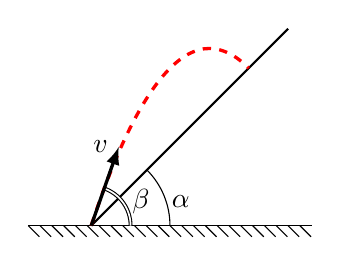
\begin{tikzpicture}[interface/.style={postaction={draw,decorate,decoration={border,angle=-45,amplitude=0.2cm,segment length=1.5mm}}},>=latex]
  \draw[interface] (0.2,0) -- (3.8,0);
  \draw[thick] (1,0) -- +(2.5,2.5);
  \draw (2,0) node[above=0.3cm,right=-0.1cm] {$\alpha$} arc
  (0:45:1cm);  
  \draw[very thick,red,dashed] (1,0) parabola bend (2.5,2.25)
  (3,2);
  \draw[double,black] (1.5,0) node[above=0.3cm,right=-0.1cm,black] {$\beta$} arc (0:atan(1/0.35):0.5cm);
  \draw[very thick,->] (1,0) -- (1.35,1) node[left] {$v$};
\end{tikzpicture}
}

\taskpic{ Утка летит по горизонтальной прямой с постоянной скоростью $u$. В
  неё бросил камень неопытный охотник, причём в момент броска
  скорость камня $v$ была направлена как раз на утку под углом $\alpha$ к
  горизонту. На какой высоте летела утка, если камень всё же попал в
  неё? }{
\begin{tikzpicture}[interface/.style={postaction={draw,decorate,decoration={border,angle=-45,amplitude=0.2cm,segment length=1.5mm}}},>=latex]
  % \draw[help lines,step=0.5] (0,0) grid (4,4);
  \draw[interface] (0.2,0) -- (3.8,0);
  \coordinate (a) at (1,0);
  \coordinate (b) at (2.5,3);
  \coordinate (c) at ($(a)!0.4!(b)$);
  \draw[dashed] (0.5,3) -- (b);
  \draw[very thick,->] (b) -- +(1,0) node[above] {$u$};
  \draw[dashed] (c) -- (b);
  \draw[very thick,->] (a) -- (c) node[left] {$v$};
  \draw ($(a)+(0.5,0)$) node[above=0.3cm,right=-0.1cm] {$\alpha$} arc
  (0:atan(2):0.5);
\end{tikzpicture}
}
